\documentclass[11pt,french]{report}
\usepackage[margin=0.7in,left=0.5in,right=0.8in]{geometry}
\usepackage[toc,page]{appendix}
\usepackage{graphicx}
\usepackage{natbib}
\usepackage{lipsum}
\usepackage{hyperref}
\usepackage[utf8]{inputenc}
\usepackage[T1]{fontenc}
\usepackage[french]{babel}
\usepackage{caption}
\usepackage[export]{adjustbox}
\usepackage[onehalfspacing]{setspace}
\usepackage{titlesec,xcolor}
\usepackage{wrapfig}
\usepackage{float}
\usepackage{rotating}
\usepackage{pifont}
\usepackage[dvipsnames]{xcolor}
\usepackage{tabularx}
\usepackage{tikz}
\usetikzlibrary{matrix}



\SetLipsumDefault{1}

\titleformat % design des titres des chapitres
{\chapter}
[display]
{\centering\normalfont\Large\scshape\bfseries}
{\rule[3pt]{0.15\linewidth}{3pt}\quad\chaptertitlename~\thechapter\quad \rule[3pt] {0.15\linewidth}{3pt}}
{0\baselineskip}%espace vertical entre chapitre et nom du chapitre
{\rule{\linewidth}{0.5pt}\break\Huge}
[\vspace{-0.5\baselineskip}\rule{\linewidth}{0.5pt}\vspace{0\baselineskip}]

\titlespacing{\chapter}{0}{0pt}{0pt}[0]

\begin{document}

\setcounter{secnumdepth}{3}
\captionsetup[figure]{margin=1.5cm,font=small,labelfont={bf},name={Figure},labelsep=colon,textfont={it}}
\captionsetup[table]{margin=1.5cm,font=small,labelfont={bf},name={Tableau},labelsep=colon,textfont={it}}

\begin{titlepage}

\begin{center}

\par
\raisebox{-.5\height}{
\includegraphics[width=7cm]{images/LogoFSR}}
\hfill{}
\raisebox{-.5\height}{
\includegraphics[width=9cm]{images/LogoDXC}} 
\par
\vspace*{1.3cm}

\linespread{1.3}\huge {\bfseries Master Informatique :}\\\Huge{Traitement Inteligent des systèmes}

\rule{\textwidth}{2pt}\\[0.2cm]
\huge{\bfseries Rapport de stage de fin d'études}
\rule{\textwidth}{2pt}\\[0.2cm]

\linespread{1.5}\huge {\bfseries Intitulé :}\\
Developpement d’une solution Power Platform pour le suivi et la gestion de la masse salariale\\[0.3cm]


\linespread{1.3}\huge {\bfseries Fait par :}\\{\huge ARCHKAK Khalil}\\[0.5cm]

\noindent \Large{\textbf{Soutenu le 21 Octobre 2022}}  \\[0.3cm]

% \linespread{2}\huge{\bfseries Encadrant :}\\
% \large{- \textbf{Abdellah IDRISII:}}\normalsize{\textbf{Professeur au sein de la faculté de science de rabat et coordinateur du master IPS}}\\
% \large{- \textbf{Ahmed EL-YAHYAOUI :}}\normalsize{\textbf{Professeur au sein de la faculté de science de rabat}}

\noindent \Large{\textbf{Devant le jury :}}  \\[0.3cm]

\begin{flushleft}
\begin{tabular}{@{}lll}

\Large{M. Abdellah IDRISSI}  &  \Large{Professeur à la Faculté des Sciences  - Rabat} & \Large{\textit{Président}}	\\[0.1cm]
\Large{M. Si Lhoussain AOURAGH }   &  \Large{Professeur à l'ENSIAS -           Rabat} & \Large{\textit{Encadrant}}	\\
\Large{M. Ez-zahout Abderrahmane}  &  \Large{Professeur à la Faculté des Sciences  - Rabat} & \Large{\textit{Examinateur}}	\\[0.1cm]

\end{tabular}
\end{flushleft}

% \begin{minipage}[t]{8cm}
% \linespread{2}\huge{\bfseries Encadrant :}\\
% \Large{\textbf{-} Abdellah IDRISSI}\\
% \Large{\textbf{-} Ahmed EL-YAHYAOUI}
% \end{minipage}
% \null\hfill
% \begin{minipage}[t]{6cm}
% \\[0.2cm]
% \linespread{2}\huge{\bfseries Maitre du stage :}\\
% \Large{\textbf{-} Adil EL-MESSARI}\\
% \end{minipage}
% \\[1.2cm]
\vspace*{0.5cm}
\textbf{\large{Année universitaire : 2021/2022}}

\end{center}

\end{titlepage}

% -------------------------------------------------------------------
% Abstract
% -------------------------------------------------------------------

\newgeometry{top=2cm,bottom=3cm,left=2.5cm,right=2.5cm}

\input{Rapport de stage PFE chez DXC/sections/remerciements}
\input{Rapport de stage PFE chez DXC/sections/resume}

% -------------------------------------------------------------------
% Contents, list of figures, list of tables
% -------------------------------------------------------------------
\newpage
\tableofcontents

\newpage
\listoffigures

% -------------------------------------------------------------------
% Main sections (as required)
% -------------------------------------------------------------------

\newpage
\input{Rapport de stage PFE chez DXC/sections/introduction}
\input{Rapport de stage PFE chez DXC/sections/description_dxc}
\input{Rapport de stage PFE chez DXC/sections/etude_generale_du_projet}
\newpage

\titleformat % design des titres des chapitres
{\chapter}
[display]
{\centering\normalfont\Large\scshape\bfseries}
{\rule[3pt]{0.15\linewidth}{3pt}\quad\chaptertitlename~\thechapter\quad \rule[3pt] {0.15\linewidth}{3pt}}
{0\baselineskip}%espace vertical entre chapitre et nom du chapitre
{\rule{\linewidth}{0.5pt}\break\Huge}
[\vspace{-0.5\baselineskip}\rule{\linewidth}{0.5pt}\vspace{0\baselineskip}]

\let\clearpage\relax% Stop LaTeX from going to a new page; and
\vspace*{5.5cm}%

\chapter{Etudes des besoins}
Le présent chapitre a pour but de définir les besoins fonctionnels et non
fonctionnels, après avoir décrit les processus métiers, et les règles de gestion.

\newpage

\section{Description du projet}
\subsection{Objectifs fonctionnels du projet}

L’objectif principal du projet est la facilitation de saisie des données ainsi que l’aide à la prise de décision, de passer d’un modèle de travail qui utilisait plusieurs fichier Excel partager avec plusieurs Equipe pour prendre la décision et s’organiser vers un modèle qui est centré sur une seul application Power Apps qui met en relation les différentes entités du system. 
\\

Dans un premier temps, il s’agit de définir de manière claire et précise les besoins et les attentes d’un système d’information permettant d’automatiser les remontées de l’équipe vers différentes entités, ainsi que la saisie des Deals, choix des Squads, l’affectation des ressources et l’affichage des statistiques dans un tableau de bord avec différents filtres. 
\\

Fournir une visibilité sur les prévisions financières au niveau du compte et du portefeuille, y compris les changements de revenus mensuels et trimestriels. Ce système devra être capable de gérer les relations clients, la saisie des différents deals pour assurer un suivi par les Services Lines, un Reporting et un suivi des indicateurs.
\\

Dans un second temps, le développement du système d’information devra permettre de garder la trace de tous les échanges afin de pouvoir établir des statistiques et prendre la décision du gain du deal.
\\

Tout au long du projet, la notion de passage à l’échelle devra être prise en compte. L’objectif à long terme de la conception et du développement d’un tel système d’information est de pouvoir être utilisé par tous les acteurs de l’entreprise.

\subsection{Fonctionnalités ciblées}

Les fonctionnalités attendues de l'application sont les suivantes :
\\

\begin{itemize}
    \item \textbf{Account Process - Ajout de la masse salariale}
    \item \textbf{Account Process - Future client}
    \item \textbf{Account Process - Roll-Off / Roll-On}
    \item \textbf{Account Process - Modification de la demande}
    \item \textbf{Account Process - Placeholder Modification de la demande}
    \item \textbf{Account Process - Consultation des soumissions}
    \item \textbf{Interlock submission with Service Line}
    \item \textbf{Interlock submission with Account}
    \item \textbf{DCT Position Level Management - Creation de demande}
    \item \textbf{DCT Position Level Management - Mise a jour de la demande}
    \item \textbf{DCT Position Level Management - Consultation des soumissions}
    \item \textbf{DCT Position Level Management - Creation des projets}
    \item \textbf{DCT Position Level Management - Mise a jour d'un projet existant}
    \item \textbf{DCT Position Level Management - Fermeture d'un projet existant}
\end{itemize}


\section{Contraintes du projet}

\subsection{Contraintes en termes de délais}
A partir de la livraison du cahier des charges, nous disposons d’environ quatre mois pour la réalisation du projet. Le délai semble court mais reste suffisant pour se concentrer sur la partie prévue pour le projet de fin d’études.

\subsection{Contraintes de sécurité}
La gestion de la sécurité est la principale contrainte de notre système. L'application doit posséder une gestion de privilèges et de niveaux d'accès pour les différents types d'utilisateurs (RH, administration, ...). Selon leur statut, le contenu des pages varie et l'accès aux informations avec un statut supérieur est interdit.

\subsection{Contraintes techniques}

Pour le développement de notre système, nous disposons d’une architecture
existante sur laquelle nous devrons baser notre application. La structure de notre système doit être extensible pour la mettre en place facilement dans les autres unités de l’entreprise. De plus, le développement devra suivre toutes les normes techniques pour une meilleure performance, maintenance et facilité de mise à jour.

\section{Etude de l'existant}

Aujourd’hui, la circulation de l’information dans une entreprise est devenue une stratégie de communication interne. En effet, lorsqu’elle circule bien, l’information favorise la communication et devient, de ce fait, facteur de cohésion, de motivation, de décision efficace et de créativité.
\\\\
Le présent système n’arrive pas à satisfaire les attentes de ses utilisateurs à cause du traitement et du fonctionnement manuelle de ce dernier, il existe plusieurs sources de données qui ne sont pas corrélées ou facilement directement liés dans une vue unique automatisée qui empêche une gestion efficace des coûts et des revenus.
\\\\
Cette incapacité à aligner étroitement les mouvements de coûts sur les mouvements de revenus a entraîné des complications et des erreurs dans le suivi et la déclaration des
action decroissance,action dans la région EMEA.
\\

Pour cette raison, Value Attainement tool a été déclaré comme besoin interne par le service Line APPS, permettant les bonnes interprétations des informations, la facilitation de saisie des données ainsi que l’aide à la prise de décision.
\\

Le workflow suivant représente le processus de gestion de demande:


\begin{figure}[!h]
    \centering
    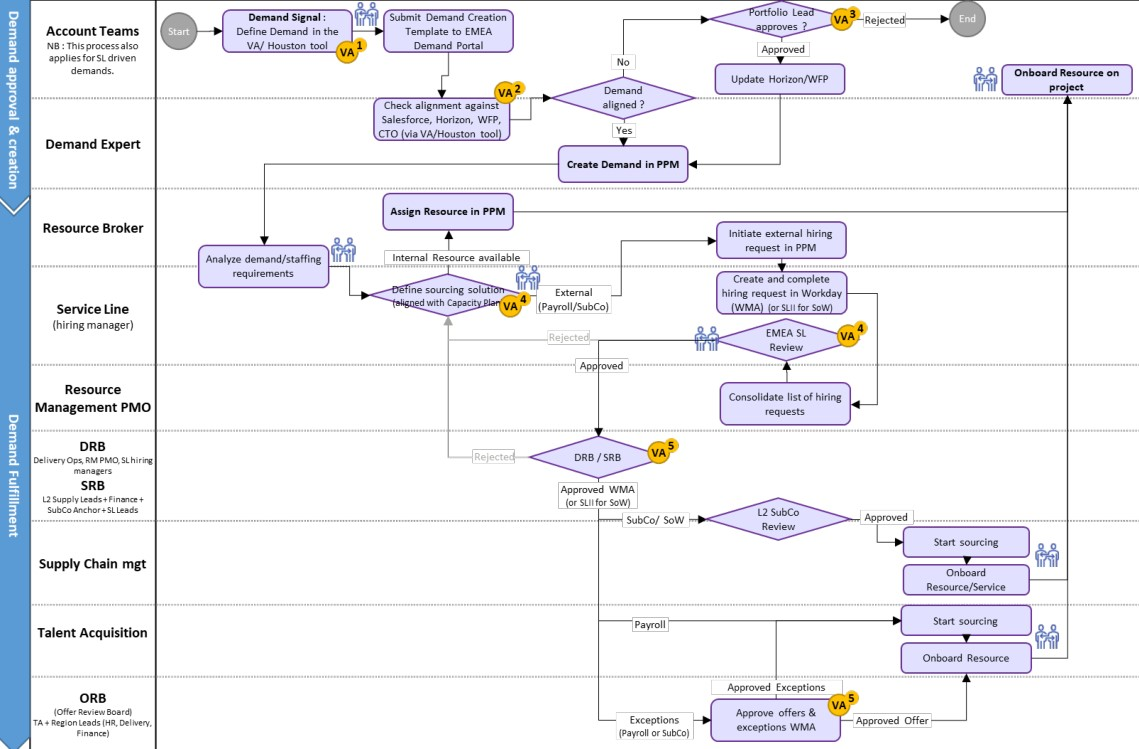
\includegraphics[scale=0.55,keepaspectratio]{Rapport de stage PFE chez DXC/figures/VA_Buisness_Process.jpg}
    \caption{Schéma descriptif de la gestion de demande}
\end{figure}

\newpage
\section{Etude Fonctionnelle}

\subsection{Objectifs fonctionnels}

Pour répondre aux besoins réels et urgents en termes de contraintes fonctionnelles, j'ai travaillé sur ces différents écrans de l'application Value Attainement Tool :
\\
\begin{itemize}
    \item \textbf{Gestion de la masse salariale:} L'application permet à l'utilisateur de gérer sa masse salariale en ajoutant ou bien réduire cette dernière mais aussi l'optimiser.
    
    \item \textbf{Consultation des soumission de la masse salariale:} Consulter les différentes soumissions sur la transformation de la masse salariale dans une seul page et aussi la sélection puis la modification possible de chaque soumission.
    
    \item \textbf{Gestion de projet DCT:} Ajout d'un nouveau projet DCT, modification de ce dernier et aussi la fermeture du projet.
    
    \item \textbf{Gestion de demande DCT:} Ajout d'un nouvelle demande, modification d'une demande.
    
    \item \textbf{Consultation des soumissions au niveau du DCT:} Consulter les différentes soumissions du DCT.
    
    \item \textbf{Consultation des soumissions au niveau du compte:} Consulter les différentes soumissions du compte.
    
\end{itemize}

\subsection{Besoins fonctionnels : Fonctionnalités}

\textbf{\color{red}Bloc fonctionnel : Gestion de la masse salariale}
    
Ce bloc fonctionnel est composé de trois écran ou bien page et il permet la gestion de la masse salariale:
\\
\begin{itemize}
    \item L'ajout d'une nouvelle demande pour l'augmentation de la masse salariale 
    \item L'ajout d'une nouvelle demande pour l'Optimisation de la masse salariale 
    \item L'ajout d'une nouvelle demande pour la réduction de la masse salariale 
\end{itemize}

\vspace{0.5cm}
\textbf{\color{red}Bloc fonctionnel : Consultation les soumission de la masse salariale:}
    
Ce bloc fonctionnel est composé d'un seul ecrant qui relie les differentes soumissions de la masse salariale:
\\
\begin{itemize}
    \item La consulation des soumission de la masse salariale
    \item La modification d'une soumission aprés sélection
    \item La modification d'un groupe de soumission
\end{itemize}

\newpage
\textbf{\color{red}Bloc fonctionnel : Gestion de projet DCT}
    
Ce bloc fonctionnel est composé de trois ecran et il permet la gestion des projet DCT: 
\\
\begin{itemize}
    \item L'ajout d'un nouveau projet DCT.
    \item La modification d'un projet DCT.
    \item La fermeture d'un projet DCT.
\end{itemize}

\vspace{0.5cm}
\textbf{\color{red}Bloc fonctionnel : Gestion de demande DCT}
    
Ce bloc fonctionnel est composé de trois ecran et il permet la gestion des demandes: 
\\
\begin{itemize}
    \item L'ajout d'une nouvelle position.
    \item La modification d'une ancienne position.
\end{itemize}

\vspace{0.5cm}
\textbf{\color{red}Bloc fonctionnel : Consultation des soumissions au niveau du DCT}
    
Ce bloc fonctionnel est composé d'un seul ecran qui relie les differentes soumissions des projets DCT.
\begin{itemize}
    \item La consultation des differentes soumission pour projet DCT.
\end{itemize}

\vspace{0.5cm}
\textbf{\color{red}Bloc fonctionnel : Validation des demande DCT}
    
Ce bloc fonctionnel est composé d'un seul ecran dans lequel on confirme et valide l'entré
\begin{itemize}
    \item L’affichage des soumission ainsi que leur validation
\end{itemize}

\subsection{Besoins non fonctionnels}

Pour la bonne gestion d'un grand projet informatique on doit prendre en compte plusieurs éléments importants comme les caractéristiques de qualités qui sont la plupart du temps des besoins implicites.
\\\\
C'est pour cela que nous avons fixé un ensemble d'objectif en termes de qualité auxquels le système doit répondre autant que possible, ces différents objectifs sont :
\\
\begin{itemize}
    \item \textbf{Fiabilité:} Le système doit fonctionner sans défaillance.
    \item \textbf{Disponibilité:} Le système doit être toujours à la disposition des utilisateurs.
    \item \textbf{Réutilisabilité:} Il doit être possible de réutiliser certains modules du
système.
    \item \textbf{Convivialité:} Le système doit être compréhensible, documenté, et son
utilisation doit être facile.
\end{itemize}
\newpage

\subsection{Acteurs}
Il s’agit de quatre acteurs principaux agissant dans le système :
\\
\begin{itemize}
    \item \textbf{BizDev:} Saisie et évolution du pipe (Deals / calcul des Revenue Mensuels
et TCV…)
    \item \textbf{Service Lines:} Compléter les données relatives aux ressources du deal 
    \item \textbf{Ressource Humaine:} Compléter la donnée relative aux ressources (Starting Date / Hiring
Date)
    \item \textbf{Finance:} Confirmer la données et verifier les budgets.
\end{itemize}


\section{Conclusion}

Dans ce chapitre j’ai donné une description du projet avec ces but et fonctionalités ciblées, les differentes contraites du projet ensuite j'ai présenté l’étude de l’existant, et les besoins fonctionnelles et non fonctionnelles du projet. 
\\
Le chapitre suivant se concentrera sur l’étude technique du projet.


\input{Rapport de stage PFE chez DXC/sections/etude_Technique}
\newpage

\titleformat % design des titres des chapitres
{\chapter}
[display]
{\centering\normalfont\Large\scshape\bfseries}
{\rule[3pt]{0.15\linewidth}{3pt}\quad\chaptertitlename~\thechapter\quad \rule[3pt] {0.15\linewidth}{3pt}}
{0\baselineskip}%espace vertical entre chapitre et nom du chapitre
{\rule{\linewidth}{0.5pt}\break\Huge}
[\vspace{-0.5\baselineskip}\rule{\linewidth}{0.5pt}\vspace{0\baselineskip}]

\let\clearpage\relax% Stop LaTeX from going to a new page; and
\vspace*{5.5cm}%

\chapter{Réalisation du projet}
Dans ce chapitre, je vais présenter la réalisation du projet. D’abord je vais exposer
les interfaces de l’application, puis nous décrirons les différentes fonctionnalités de ces dernières.

\newpage

\section{Interface d'acceuil}

\begin{figure}[!h]
    \centering
    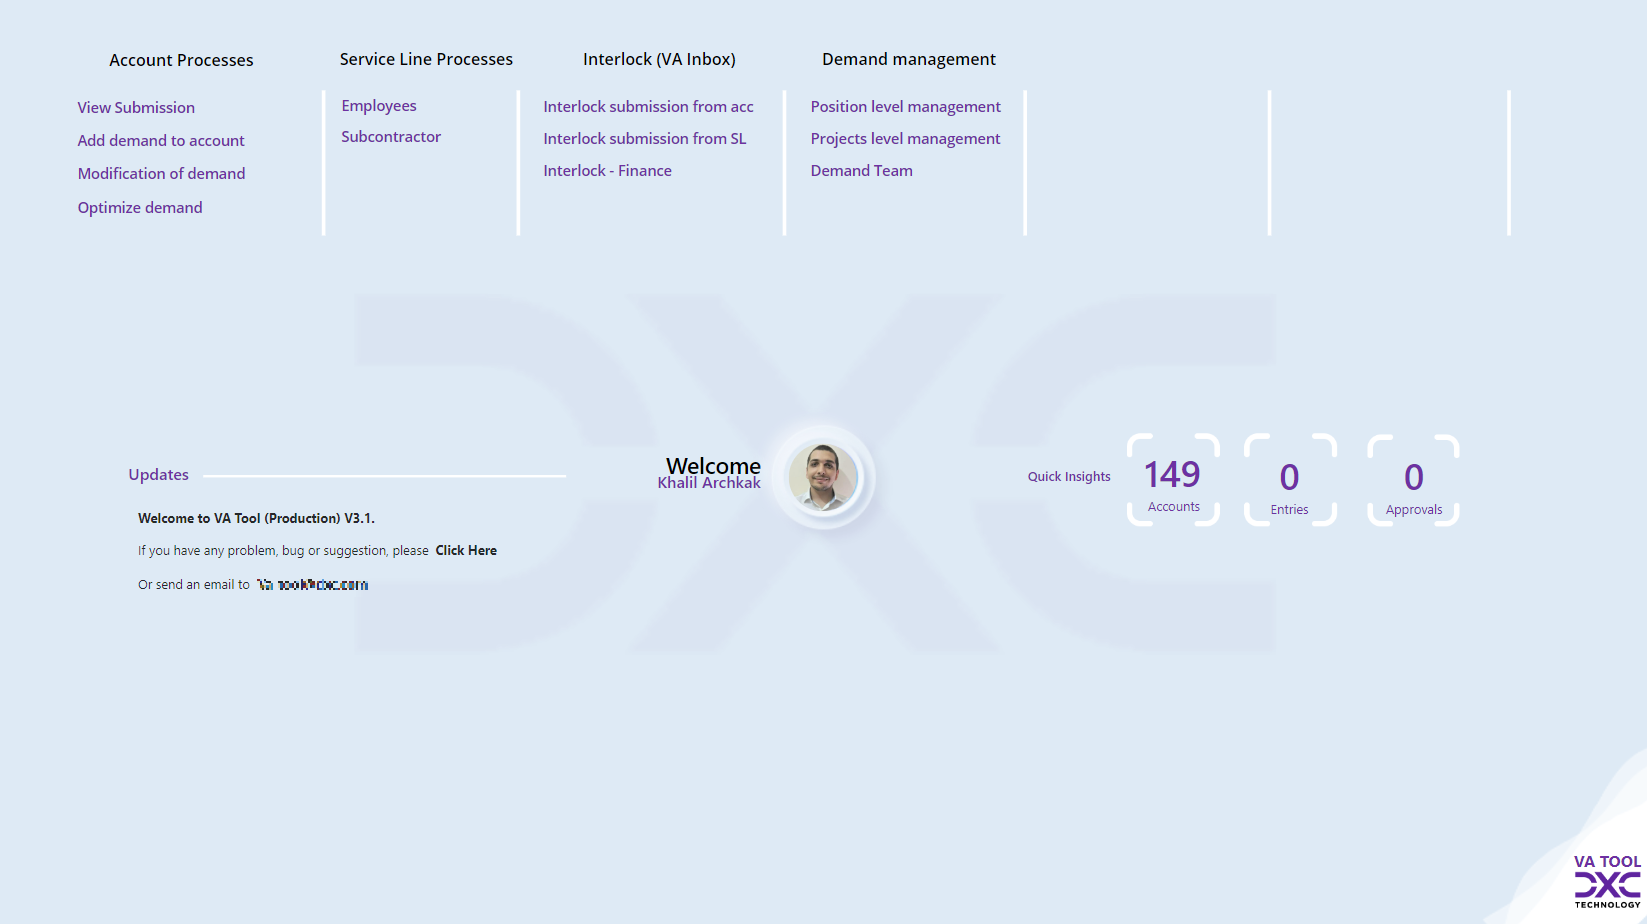
\includegraphics[scale=0.4,keepaspectratio]{Rapport de stage PFE chez DXC/figures/Home_Page.png}
    \caption{Interface d'accueil}
\end{figure}

La page d'accueil regroupe les différentes procédures possibles que propose l'application dans un menu verticale à savoir les procédures en relation avec les comptes, le service line, l'interlock de ces deux dernier mais aussi la gestion des demandes.
\\[0.3cm]
Elle contient aussi un aperçu rapide du nombre de compte affecté pour l'utilisateur, le nombre d'entré saisie par l'utilisateur mais aussi le nombre d'entré validé par ce dernier.
\\[0.3cm]
On peut aussi etre re-directionner vers une application d'aide ou bien envoyer un email en cas de problem a la mailbox de support. 

\newpage
\section{Ajout de masse salariale}
Pour l'ajout de masse salariale au niveau du compte 4 option se presente :

\begin{itemize}
    \item \textbf{Compte existant:} Le compte auxquelle on ajoute une demande existe déja en tant que client
    \item \textbf{New logo:}  Le compte auxquelle on souhaite ajouté une demande n'est pas encore un client
    \item \textbf{Roll-Off\Roll-on:} L'employé qu'on souhaite ajouter se trouve déja dans un autre projet et va changer ce dernier
    \item \textbf{PlaceHolder - add demand:} L'utilisateur souhaite créer une entré pour un future besoin
\end{itemize}

\subsection{Compte existant}

\begin{figure}[!h]
    \centering
    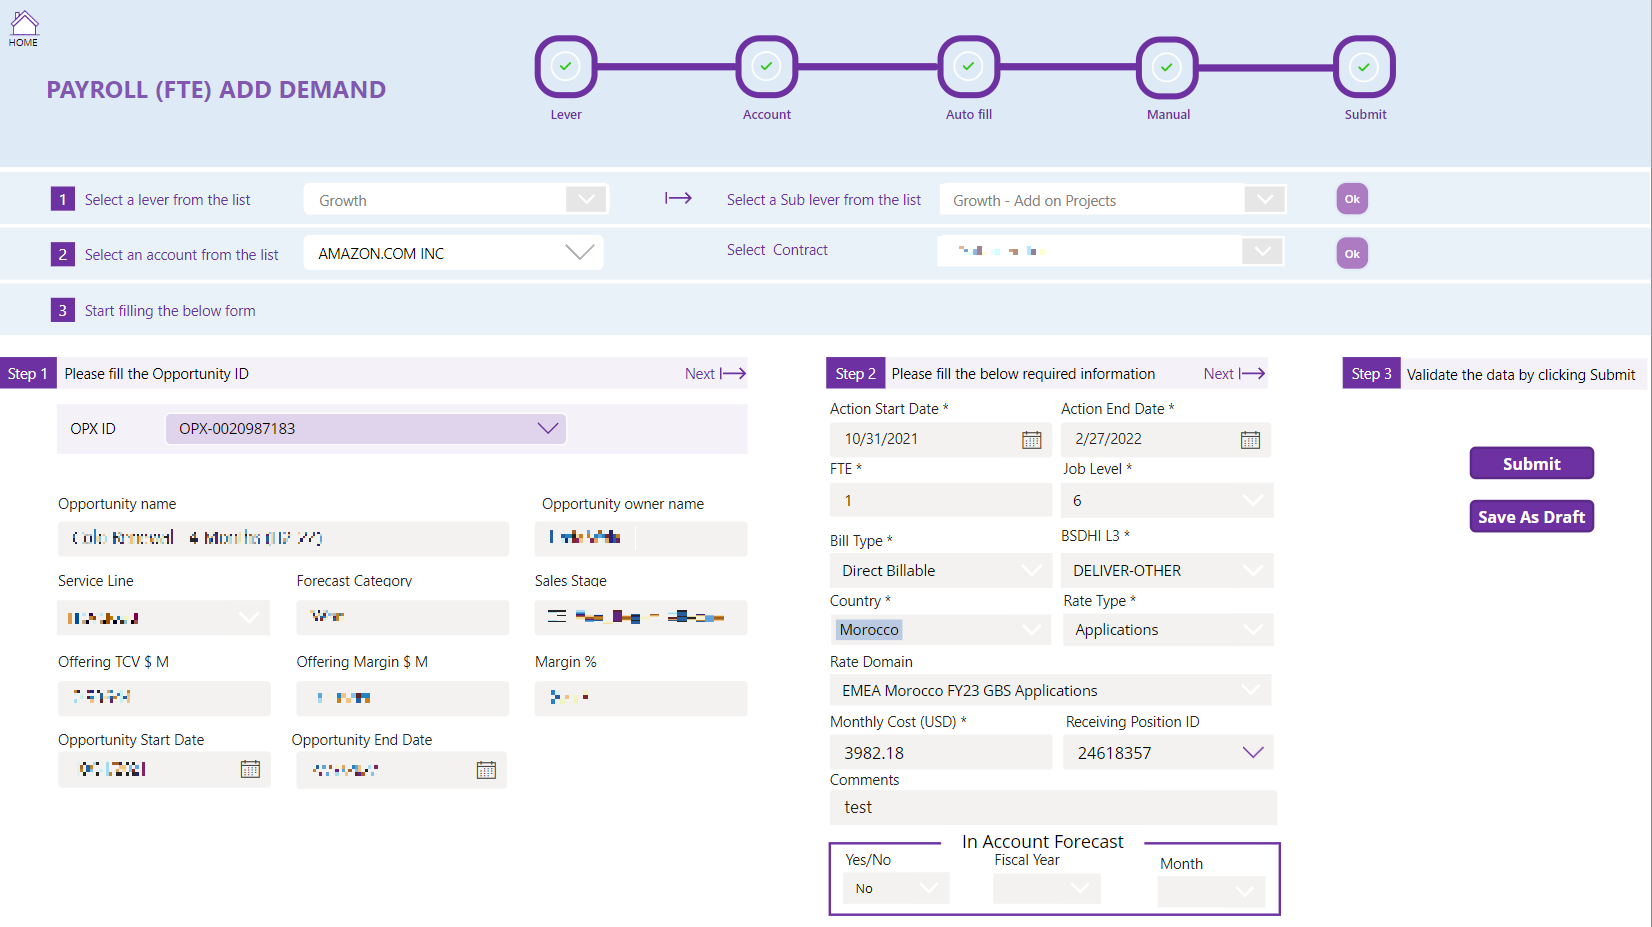
\includegraphics[scale=0.4,keepaspectratio]{Rapport de stage PFE chez DXC/figures/existin_account.png}
    \caption{Ajout de demande - Compte existant}
\end{figure}

L'utilisateur doit sélectionner le compte auxquelles il souhaite ajouter une demande, ensuite il doit saisir l'OPX-ID qui représente un identificateur pour une opportunité, ensuite toutes les informations de la première étape sont automatiquement remplies, puis l'utilisateur doit saisir les différentes informations de la deuxième étape en respectant les différentes contraintes. 
\\[0.3cm]
Deux options s’offrent à l'utilisateur pour saisir l’entrer il peut soit la soumettre directement ou bien l'enregistrer en tant que brouillon pour s'assurer des informations et la soumettre après.

\newpage
\subsection{New Logo}

\begin{figure}[!h]
    \centering
    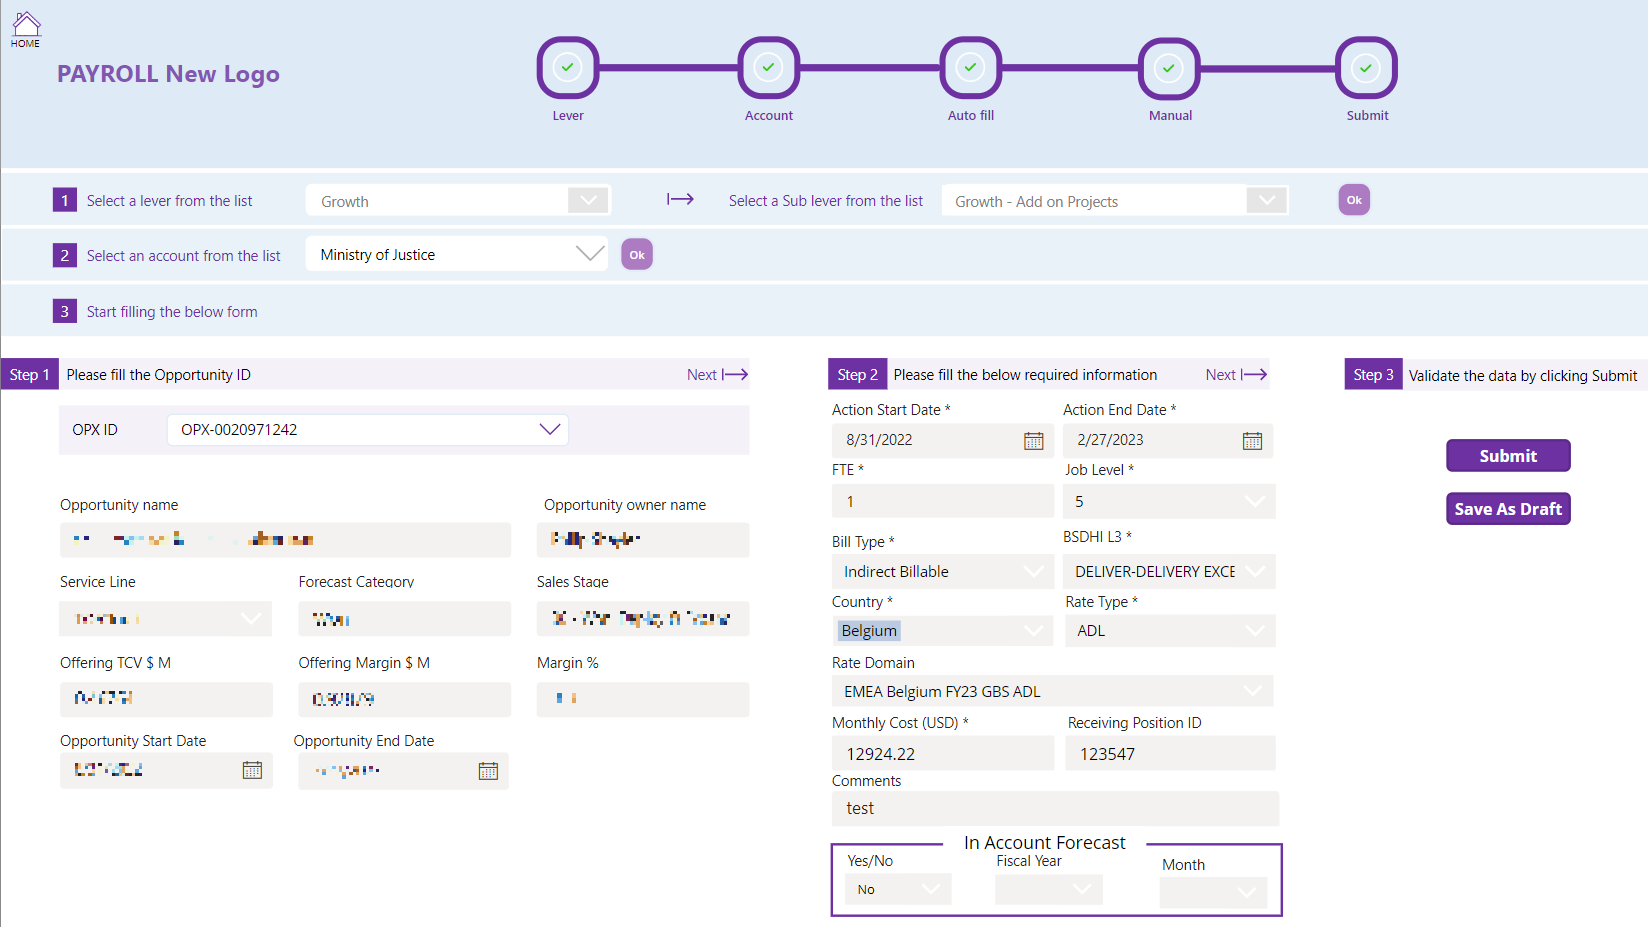
\includegraphics[scale=0.4,keepaspectratio]{Rapport de stage PFE chez DXC/figures/New_Logo.png}
    \caption{Ajout de demande - New Logo}
\end{figure}

Ce formulaire fonctionne de la meme facon que le precedent la seul difference est dans le choix du compte, dans ce dernier le choix du compte est fait a travers le contrat SalesForce car le compte n'est pas encore un client de DXC d'ou le nom de New Logo.

\subsection{Roll-Off / Roll-On}

\begin{figure}[H]
    \centering
    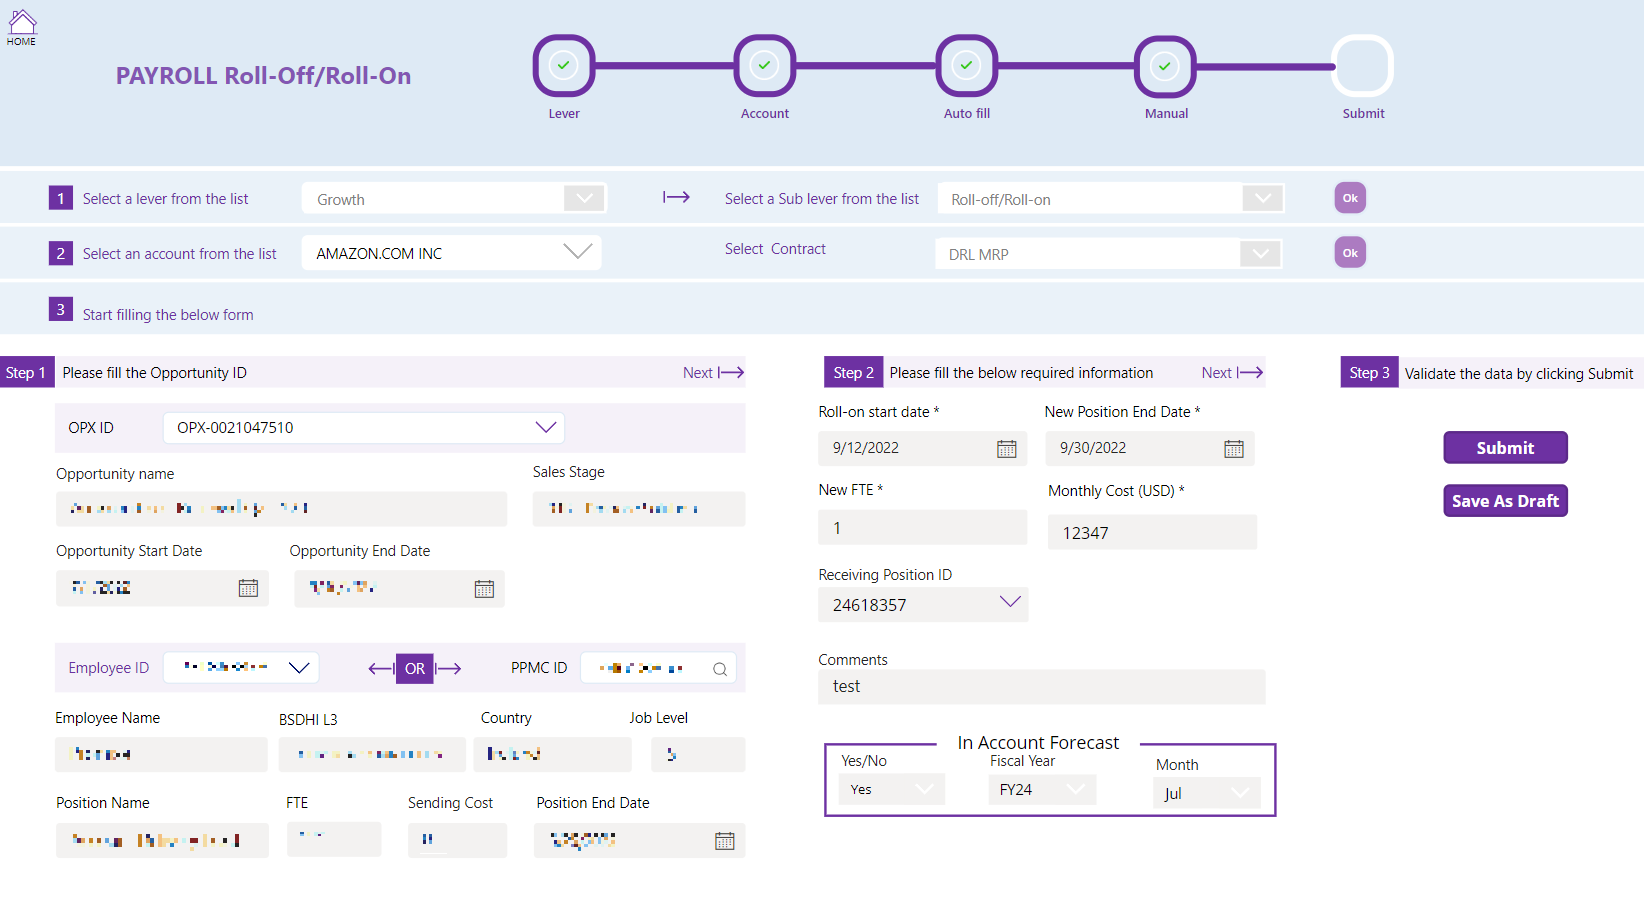
\includegraphics[scale=0.4,keepaspectratio]{Rapport de stage PFE chez DXC/figures/rolloff_rollon.png}
    \caption{Ajout de demande - Roll-Off / Roll-On}
\end{figure}

Pour le "Roll-Off/Roll-On", Un employé change de projet en restant avec le meme client.
\\
Dans la 1er etape l'utilisateur doit saisire l'OPX-ID mais aussi l'identificateur de l'employé qui vas faire la transition, ensuite il remplis les information necessaire dans la deuxieme étape tout en resepectant les differrentes contrainte, ensuite de la meme maniere il peut soit soumettre ou sauvegarder l'entré comme brouillon

\subsection{PlaceHolder - Add Demand}

\begin{figure}[H]
    \centering
    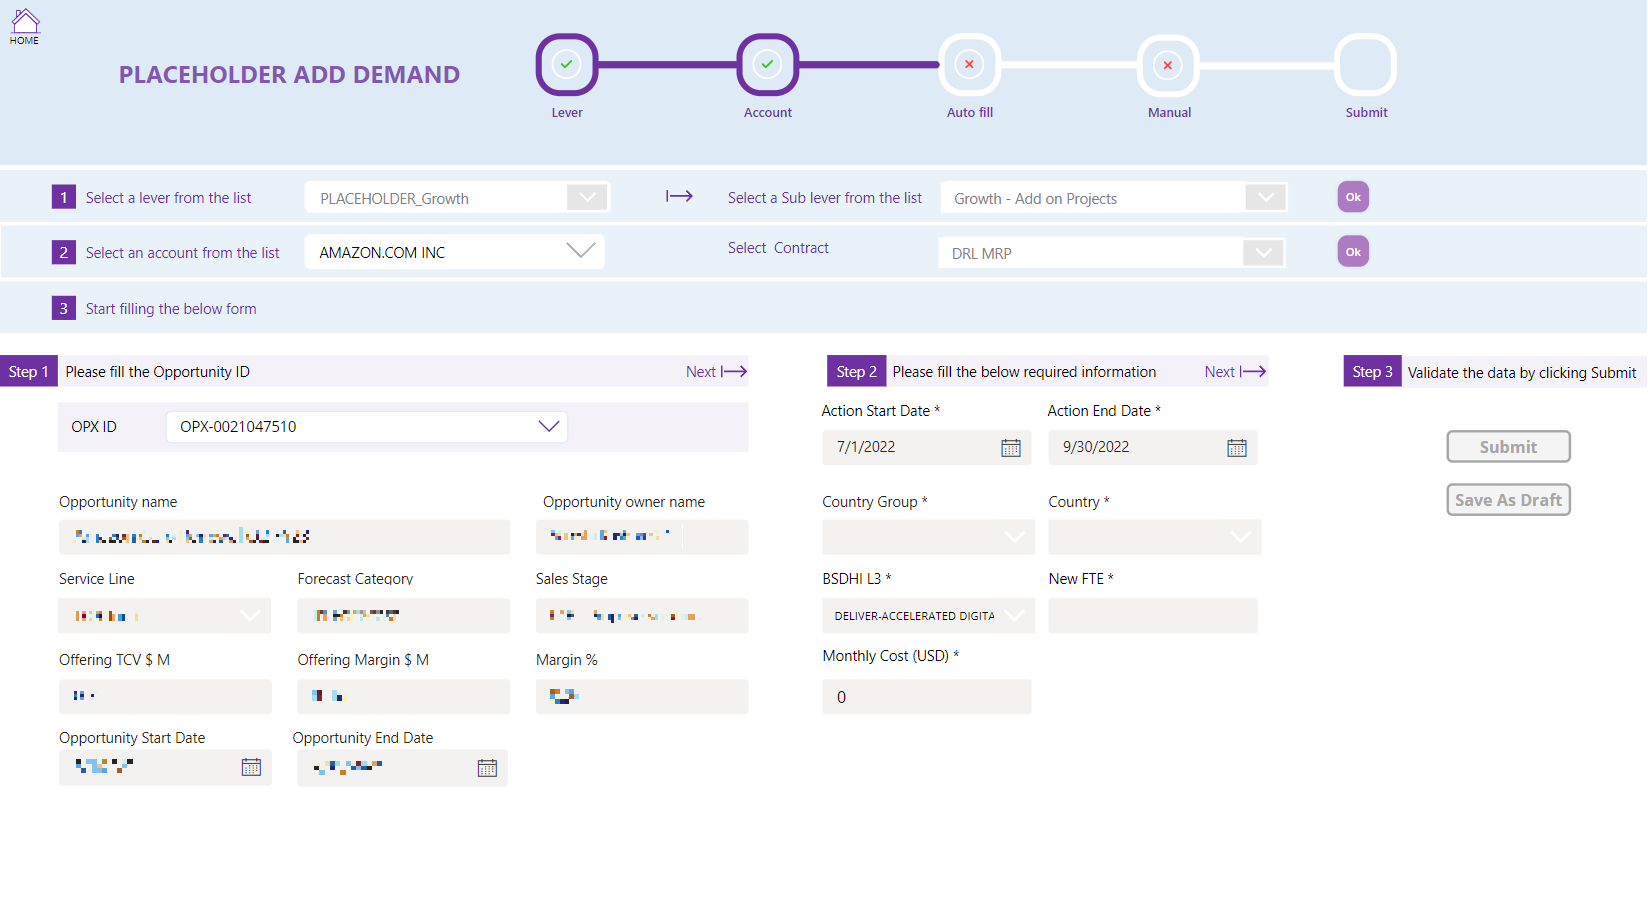
\includegraphics[scale=0.4,keepaspectratio]{Rapport de stage PFE chez DXC/figures/Placeholder_add_demand.png}
    \caption{Ajout de demande - Placeholder Add Demand}
\end{figure}

Pour les placeholders se sont des submission pour un future besoin, aprés avoir créer un placeholder ce dernier peut etre convertis ensuite en une entré VA dans la vue de submission, La soumission de cette entré se fait de la meme maniére que pour l'ajout de demande. 



\newpage

\titleformat % design des titres des chapitres
{\chapter}
[display]
{\centering\normalfont\Large\scshape\bfseries}
{\rule[3pt]{0.15\linewidth}{3pt}\quad\chaptertitlename~\thechapter\quad \rule[3pt] {0.15\linewidth}{3pt}}
{0\baselineskip}%espace vertical entre chapitre et nom du chapitre
{\rule{\linewidth}{0.5pt}\break\Huge}
[\vspace{-0.5\baselineskip}\rule{\linewidth}{0.5pt}\vspace{0\baselineskip}]

\let\clearpage\relax% Stop LaTeX from going to a new page; and

\chapter{Conclusion Générale}


DXC Technology dispose de plusieurs départements de différents services, L’un de ses départements est le BizDev (le service financier), qui est responsable de la gestion des appels d’offres, création des équipes et l’affectation des ressources. Ce dernier à déclarer un besoin urgent causé par la mauvaise gestion des effectifs et ressources.
\\\\
L’objectif de notre projet est de développer une application WEB de gestion de masse salariale. L’application vient comme solution aux différents problématiques que rencontre le service financier de DXC Technology lors de la gestion de ces derniers : La saisie manuelle est des informations, l’utilisation excessive des fichiers Excel, le manque de centralisation de l’information.
\\\\
L’application web « VA-TOOL » crée une harmonie entre les équipes en centralisons tout le processus de gestion des ressources en une seul application hébergé dans le cloud et accessible a toute personne de l’environnement DXC.
\\\\
Ce stage de fin d’étude en entreprise était pour moi une fabuleuse occasion pour tester et de mettre en pratique mes compétences et capacités acquises durant notre formation a la faculté de science de Rabat.
\\\\
Concernant le coté technique ce stage m’a permis de découvrir une nouvelle technologie à savoir Power Platform, une technologie conçue pour faciliter et la gestion et le développement d’un projet.
\\\\
Pour ce qui est des perspectives notre projet est dans ces premières phases, il reste alors d’ajouter d’autre acteurs pour clore la boucle, à savoir les équipes RH et Finance.
\\\\
Enfin je remercie encore La faculté de science de Rabat et DXC Technology Maroc pour cette opportunité qui m'a ouvert les portes du monde professionnel et m'a permis d'améliorer mes capacités à tous les niveaux.

\printbibliography
\printbibliography

% -------------------------------------------------------------------
% Bibliography
% -------------------------------------------------------------------

\bibliographystyle{plain} 
\bibliography{bibliographie}{}


% -------------------------------------------------------------------
% Appendices
% -------------------------------------------------------------------

% \begin{appendices}
% % \input{sections/appendixA.tex}
% % \input{sections/appendixB.tex}
% \end{appendices}

\end{document}
